\documentclass[11pt]{article}

\usepackage[margin=1in]{geometry}
\usepackage{amsmath,amssymb,amsthm}
\usepackage{graphicx}
\usepackage[hidelinks]{hyperref}

\newtheorem{theorem}{Theorem}

\newcommand{\ellone}{\ell_1}
\newcommand{\cnull}{c_0}
\newcommand{\Xiw}{X_{\mathbf{iw}}}

\title{A Literature-Implied Negative Answer to the Asymptotic-\texorpdfstring{\(\cnull\)}{c0} Subspace Question}
\author{Status packet for arXiv:1607.03587 and arXiv:1902.10092}
\date{June 14, 2026}

\begin{document}
\maketitle

\section*{Source and Original Problem}

The source paper is Freeman--Odell--Sari--Zheng,
\emph{On spreading sequences and asymptotic structures}, arXiv:1607.03587
\cite{FOSZ}. Problem 4.5 asks whether the following hypotheses force either an
asymptotic-\(\cnull\) subspace or a subspace with separable dual:
\[
  \ellone \not\hookrightarrow X
  \quad\text{and}\quad
  \text{every weakly-null spreading model in }X\text{ is equivalent to }\cnull.
\]

\begin{center}

\includegraphics[width=\textwidth]{figures/open_problem_crop.png}
\end{center}

This packet records a negative answer only to the first question, the existence
of an asymptotic-\(\cnull\) subspace.

\section*{Supporting Literature}

The supporting paper is Argyros--Motakis,
\emph{On the complete separation of asymptotic structures in Banach spaces},
arXiv:1902.10092 \cite{AM}. Their Theorem A constructs a reflexive Banach
space \(\Xiw\).

\begin{center}
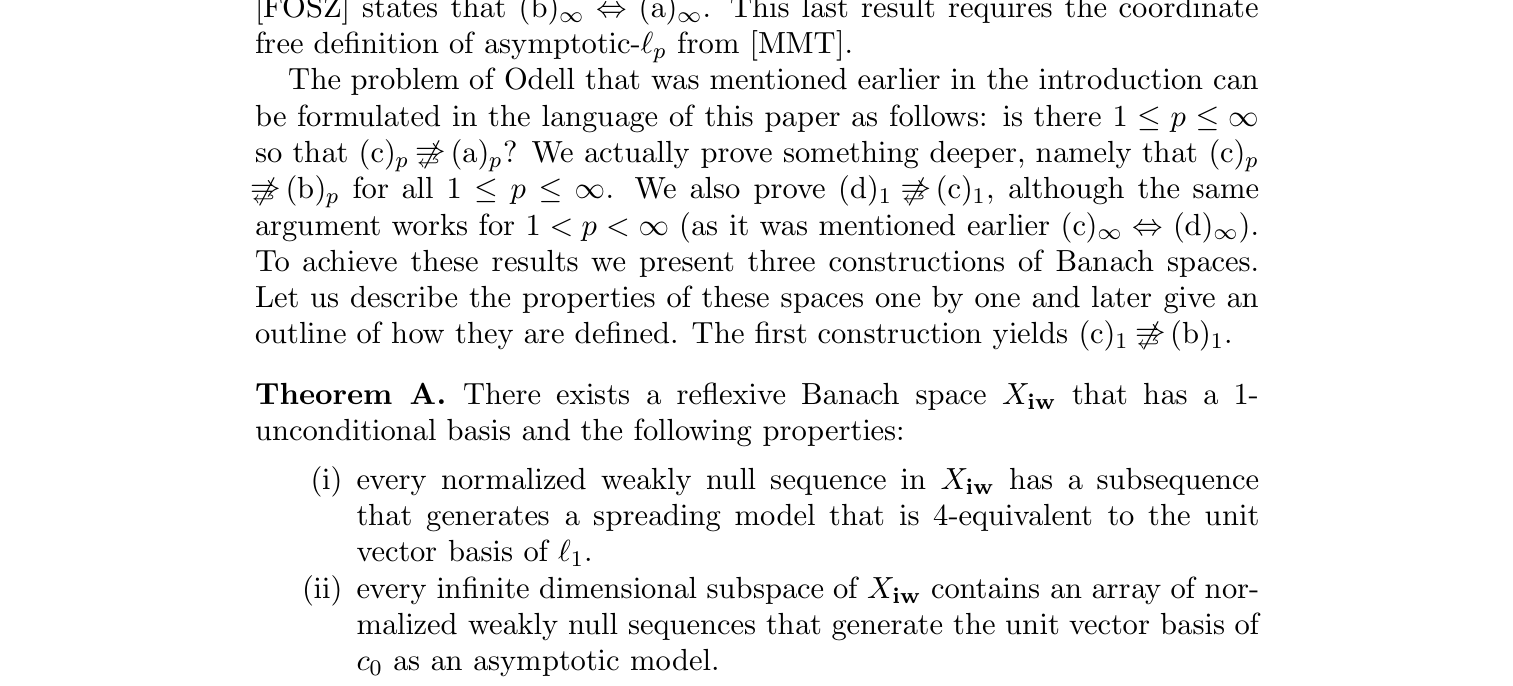
\includegraphics[width=\textwidth]{figures/supporting_theorem_a_crop.png}
\end{center}

Their Theorem C gives the relevant behavior of the dual \(\Xiw^*\).

\begin{center}

\includegraphics[width=\textwidth]{figures/supporting_theorem_c_crop.png}
\end{center}

The same paper explicitly states in Section 10 that \(\Xiw^*\) has no
asymptotic-\(\cnull\) subspace.

\begin{center}
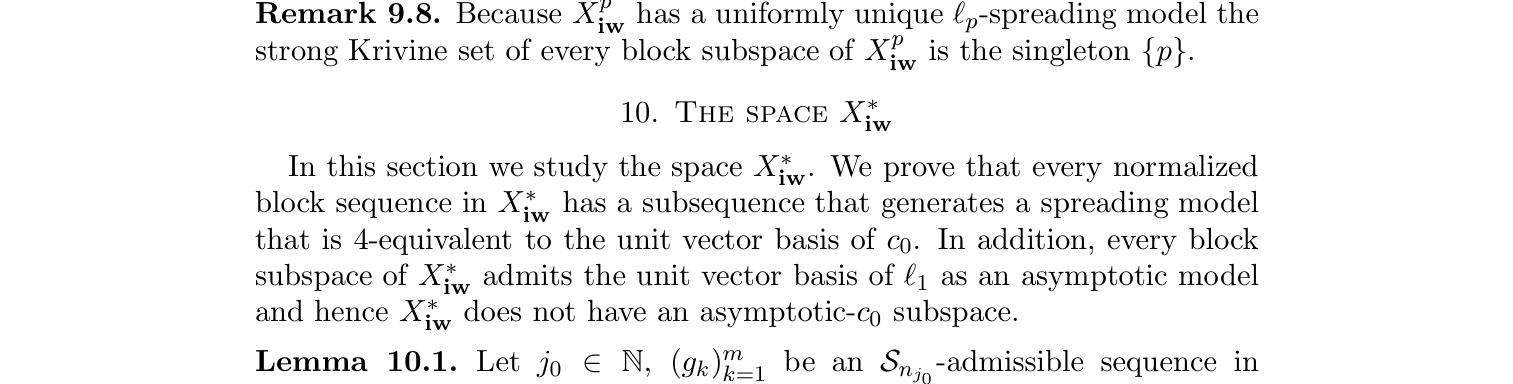
\includegraphics[width=\textwidth]{figures/supporting_no_asymptotic_c0_crop.png}
\end{center}

\section*{Idea of the Proof}

The only identification needed beyond the cited construction is a basic
feature of spreading models: if a sequence generates a spreading model, then
all of its subsequences generate the same spreading model. Argyros--Motakis
prove that every normalized weakly-null sequence in \(\Xiw^*\) has a subsequence
generating \(\cnull\). Therefore any weakly-null sequence which already
generates a spreading model can only generate \(\cnull\). Since \(\Xiw^*\) is
reflexive and has no asymptotic-\(\cnull\) subspace, it gives the promised
negative answer to the first half of Problem 4.5.

\section*{Theorem}

\begin{theorem}
The first question in \cite[Problem 4.5]{FOSZ} has a negative answer. More
precisely, there is a Banach space \(Z\) such that \(\ellone\) does not embed
into \(Z\), every spreading model generated by a normalized weakly-null
sequence in \(Z\) is equivalent to the unit vector basis of \(\cnull\), and
\(Z\) contains no asymptotic-\(\cnull\) subspace.
\end{theorem}

\begin{proof}
Let \(Z=\Xiw^*\), where \(\Xiw\) is the Argyros--Motakis space from
\cite{AM}. By \cite[Theorem A]{AM}, \(\Xiw\) is reflexive. Hence \(Z=\Xiw^*\)
is reflexive as well. Since every closed subspace of a reflexive space is
reflexive and \(\ellone\) is not reflexive, \(\ellone\) does not embed into
\(Z\).

We next verify the spreading-model hypothesis from \cite[Problem 4.5]{FOSZ}.
Let \((z_n)\) be a normalized weakly-null sequence in \(Z\) which generates a
spreading model \((e_n)\). By \cite[Theorem C(i)]{AM}, \((z_n)\) has a
subsequence \((z_{n_k})\) generating a spreading model 4-equivalent to the unit
vector basis of \(\cnull\). But every subsequence of a sequence that generates a
spreading model generates the same spreading model. Thus \((e_n)\) is
equivalent to the unit vector basis of \(\cnull\).

Finally, Argyros--Motakis state in Section 10 of \cite{AM} that
\(\Xiw^*\) does not have an asymptotic-\(\cnull\) subspace. Therefore \(Z\)
satisfies the hypotheses of \cite[Problem 4.5]{FOSZ} while failing the
asymptotic-\(\cnull\) subspace conclusion.
\end{proof}

\section*{Scope and Limitations}

This is a literature-implied answer, not an original construction from this
run. The supporting paper does not appear to state that it is answering
\cite[Problem 4.5]{FOSZ}; the implication is obtained by combining its Theorem
C and Section 10 with the standard subsequence property of spreading models.

The second question in \cite[Problem 4.5]{FOSZ}, asking for a subspace
\(Y\subset X\) with \(Y^*\) separable, is not answered negatively here. Indeed,
the example \(Z=\Xiw^*\) is reflexive and comes from a space with a countable
basis, so \(Z^*\cong \Xiw\) is separable.

The run indexes were searched for arXiv:1607.03587, the source title,
\(\cnull\) spreading-model keywords, asymptotic-\(\cnull\), and arXiv:1902.10092
before promotion. A bounded web search on June 14, 2026 found the separate
follow-up arXiv:1611.04443 for the source paper's Argyros conditional-spreading
problem; no existing run packet was found for this implication from
arXiv:1902.10092.

\section*{Human Review Recommendation}

Check the identification between the source problem's hypothesis and
\cite[Theorem C(i)]{AM}, especially the use of subsequences of sequences that
already generate a spreading model. Also check that the supporting paper's
``no asymptotic-\(\cnull\) subspace'' statement is being used with the same
coordinate-free meaning intended in \cite[Problem 4.5]{FOSZ}.

\begin{thebibliography}{9}

\bibitem{FOSZ}
D. Freeman, E. Odell, B. Sari, and B. Zheng,
\emph{On spreading sequences and asymptotic structures},
Studia Mathematica 240 (2018), no. 1, 69--91; arXiv:1607.03587.

\bibitem{AM}
S. A. Argyros and P. Motakis,
\emph{On the complete separation of asymptotic structures in Banach spaces},
Advances in Mathematics 362 (2020), 106962; arXiv:1902.10092.

\end{thebibliography}

\end{document}
